%%%%%%%%%%%%%%%%%%%%%%%%%%%%%%%%%%%%%%%%%
% Stylish Article
% LaTeX Template
% Version 2.2 (2020-10-22)
%
% This template has been downloaded from:
% http://www.LaTeXTemplates.com
%
% Original author:
% Mathias Legrand (legrand.mathias@gmail.com) 
% With extensive modifications by:
% Vel (vel@latextemplates.com)
%
% License:
% CC BY-NC-SA 3.0 (http://creativecommons.org/licenses/by-nc-sa/3.0/)
%
%%%%%%%%%%%%%%%%%%%%%%%%%%%%%%%%%%%%%%%%%

%----------------------------------------------------------------------------------------
%	PACKAGES AND OTHER DOCUMENT CONFIGURATIONS
%----------------------------------------------------------------------------------------

\documentclass[fleqn,10pt]{SelfArx} % Document font size and equations flushed left

\usepackage[fontset=none]{ctex}
\setCJKmainfont{Noto Serif CJK SC}
\setCJKsansfont{Noto Serif CJK SC}
\setCJKmonofont{Noto Sans CJK SC}

%----------------------------------------------------------------------------------------
%	COLUMNS
%----------------------------------------------------------------------------------------

\setlength{\columnsep}{0.55cm} % Distance between the two columns of text
\setlength{\fboxrule}{0.75pt} % Width of the border around the abstract

%----------------------------------------------------------------------------------------
%	COLORS
%----------------------------------------------------------------------------------------

\definecolor{color1}{RGB}{0,0,90} % Color of the article title and sections
\definecolor{color2}{RGB}{0,20,20} % Color of the boxes behind the abstract and headings

%----------------------------------------------------------------------------------------
%	HYPERLINKS
%----------------------------------------------------------------------------------------

\usepackage{hyperref} % Required for hyperlinks

\hypersetup{
	hidelinks,
	colorlinks,
	breaklinks=true,
	urlcolor=color2,
	citecolor=color1,
	linkcolor=color1,
	bookmarksopen=false,
	pdftitle={Title},
	pdfauthor={Author},
}

%----------------------------------------------------------------------------------------
%	ARTICLE INFORMATION
%----------------------------------------------------------------------------------------

\JournalInfo{基础物理学实验A3} % Journal information
\Archive{} % Additional notes (e.g. copyright, DOI, review/research article)

\PaperTitle{实验报告} % Article title

\Authors{} % Authors
\affiliation{} % Author affiliation

\Keywords{} % Keywords - if you don't want any simply remove all the text between the curly brackets
\newcommand{\keywordname}{Keywords} % Defines the keywords heading name

%----------------------------------------------------------------------------------------
%	ABSTRACT
%----------------------------------------------------------------------------------------

\Abstract{本实验通过对耦合弹簧振子的研究,用实验的方法测试耦合摆装置的固有频率、振动波长,并借此验证色散关系。另外,本实验还测定并给出了通频范围之外的振动在耦合摆中的传播规律。} 

%----------------------------------------------------------------------------------------

\begin{document}

\maketitle % Output the title and abstract box

\tableofcontents % Output the contents section

\thispagestyle{empty} % Removes page numbering from the first page

%----------------------------------------------------------------------------------------
%	ARTICLE CONTENTS
%----------------------------------------------------------------------------------------

\section{实验原理} % The \section*{} command stops section numbering

我们将数量较少的耦合摆的模型的情况直接推广到N耦合摆。我们可以预测,对于N耦合摆,具有N个固有角频率$\omega_k$和N个振动模式,对应模数$\kappa=0\~(N-1)$。对于其中的每一个摆球,可知:当模数$\kappa=0$的时候,所有单摆都在以固有角频率$\omega_0$做同相位简谐振动,而当模数$\kappa=1\~(N-1)$的时候,摆球的振幅呈现$x=A\sin(kn-\phi)$的关系。

通过计算N耦合摆中各个摆球的动力学方程,我们可以得到N耦合摆的色散关系($\omega\~ k$关系):
\begin{equation}
	\omega=\sqrt{\omega_p^2+4\omega_s^2\sin^2(\frac{k}{2})}=\sqrt{\omega_p^2+4\omega_s^2\sin^2(\frac{\pi\kappa}{2N})}
	\label{eq:1}
\end{equation}

本实验一共15个摆球,根据实验器材数据,理论上的$\omega_p=4.43rad/s$,$\omega_s=11.3rad/s$。根据\ref{eq:1},取$N=15$,对不同的$\kappa$带入,得到固有频率的理论值:

\begin{table}[htbp]
\centering
\begin{tabular}{|l|l|l|}
\hline
$f(Hz)$ & $f(Hz)$ & $f(Hz)$ \\ \hline
0.705        & 0.799        & 1.03         \\ \hline
1.32         & 1.62         & 1.93         \\ \hline
2.23         & 2.51         & 2.76         \\ \hline
2.99         & 3.19         & 3.36         \\ \hline
3.49         & 3.59         & 3.65         \\ \hline
\end{tabular}
\caption{固有频率理论值}
\label{tab:1}
\end{table}

%------------------------------------------------

\section{实验操作及数据处理}

\subsection{固有频率的测定}

先测定固有频率,本实验使用传感器来将摆球的位置信息转化为电压信息。用小锤轻轻敲击最右端摆球,使摆球起振。理论来说,任意一个摆球的振动都是不同峰值的固有频率振动的叠加,因此我们采用傅里叶变换(示波器自身能完成傅里叶变换)的方式就可以得到叠加成这一振动的频率,其中波幅较大的频率就认为是耦合摆的固有频率。

使用上述方法,测定出耦合摆的10个固有频率如下表:

\begin{table}[htbp]
\centering
\begin{tabular}{|l|l|l|}
\hline
$f(Hz)$ & $f(Hz)$ & $f(Hz)$ \\ \hline
0.732        & 0.820        & 1.022        \\ \hline
1.280        & 1.580        & 1.868        \\ \hline
2.144        & 2.416        & 2.592        \\ \hline
2.876        &              &              \\ \hline
\end{tabular}
\caption{固有频率测量值}
\label{tab:2}
\end{table}

可以看到,测量值与对应的理论值之间相近,但是测量值偏大。这是由于弹簧自身损耗,每个摆球不完全相同,计算数据不完全准确等多种原因造成的。

\subsection{验证耦合摆的色散关系}

跟据\ref{eq:1},为了验证色散关系,我们需要一系列的$k$值。而考虑每一个摆球在固有频率下的振动,根据理论部分的分析,摆球的振幅存在$x=A\sin(kn-\phi)$的关系。需要注意的是,A的正负包含相位的信息,我们设定0号摆球为正,相位与其相反为负。实际实验操作中,需要肉眼观察,若相邻两球运动方向一致,说明符号一致;若相邻两球运动方向相反,说明从相反的球开始,振幅变为负。我们选取了4个实验测定的固有频率值来作为驱动频率,测定同驱动频率下振幅的情况,并拟合得到$k$。(顺带由$k$可以得到振动波长$\lambda$)

对于$1.022Hz$的情况,测定结果如图\ref{fig:1022}。我们使用python的scipy包做任意函数拟合(实际上原理上是在给定的优化区间和步数内做一个最小二乘法的优化)。拟合得到$k=0.415$,$lambda=15.1$。(由于电压正比于位置,尽管这里得到的$k$实际上是一个电压的负一次方的量纲,$\lambda$实际上是电压的量纲,但可以代表位置量纲下的信息(差一个系数)。这不影响频率相关的计算)

\begin{figure}[htbp]
	\centering
	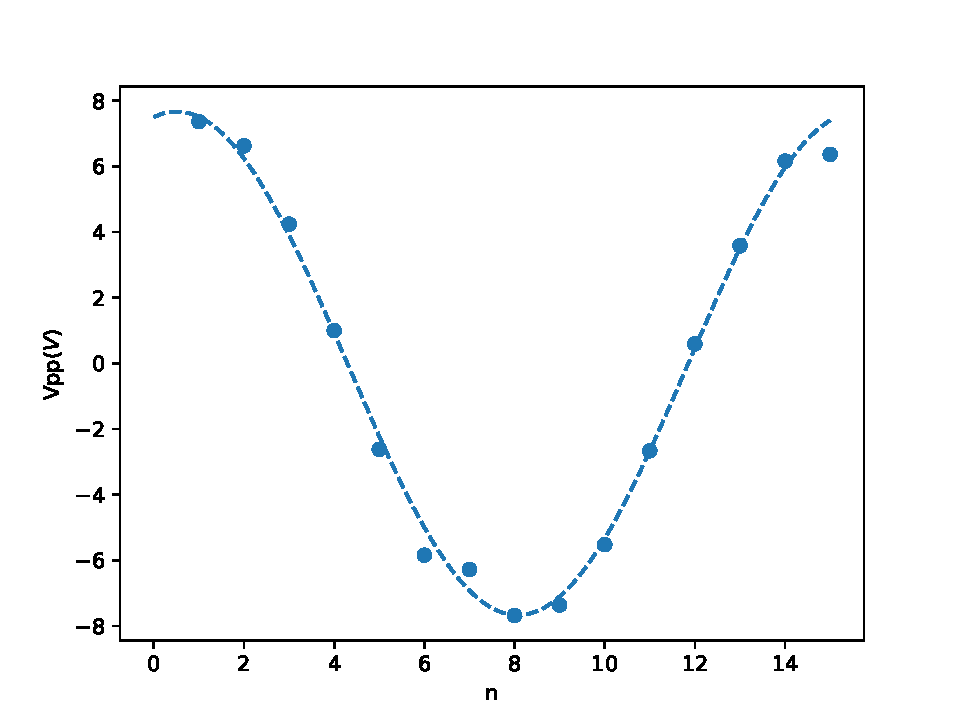
\includegraphics[width=\linewidth]{1022.pdf}
	\caption{$1.022Hz$}
	\label{fig:1022}
\end{figure}

对于$1.28Hz$的情况,测定结果如图\ref{fig:1280}。拟合得到$k=0.627$,$\lambda=10.0$。

\begin{figure}[htbp]
	\centering
	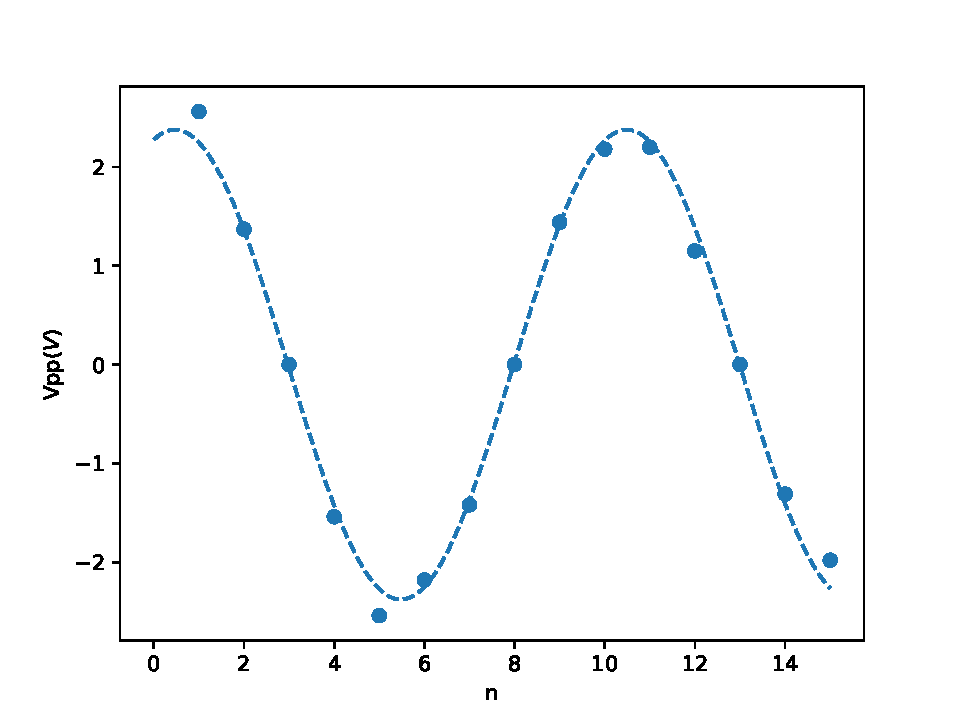
\includegraphics[width=\linewidth]{1280.pdf}
	\caption{$1.280Hz$}
	\label{fig:1280}
\end{figure}

对于$1.58Hz$的情况,测定结果如图\ref{fig:1580}。拟合得到$k=0.837$,$\lambda=7.51$。

\begin{figure}[htbp]
	\centering
	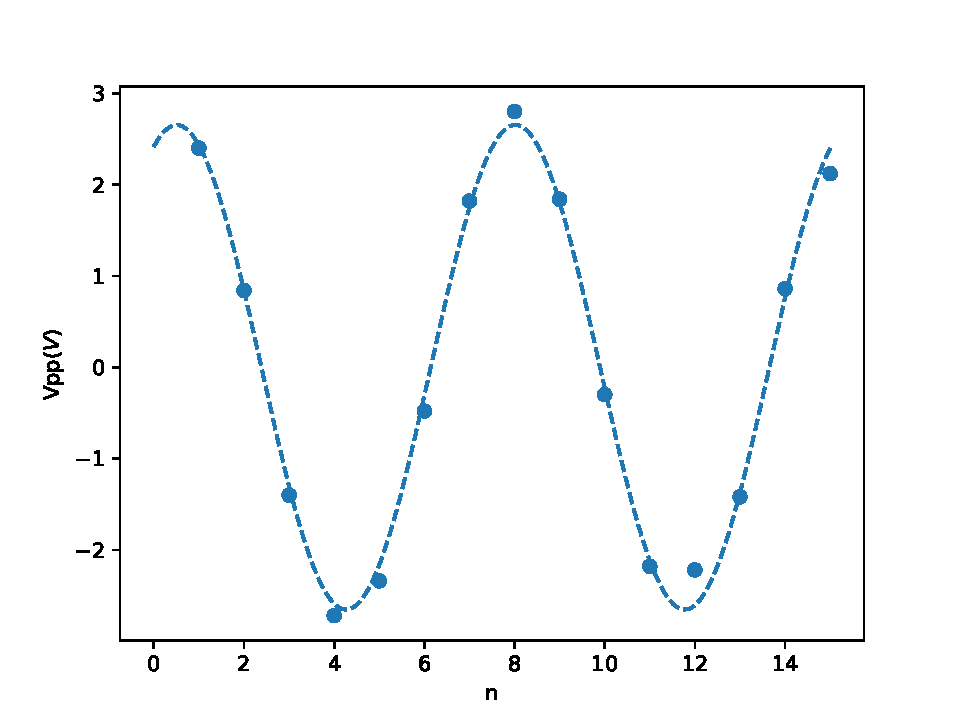
\includegraphics[width=\linewidth]{1580.pdf}
	\caption{$1.580Hz$}
	\label{fig:1580}
\end{figure}

对于$2.14Hz$的情况,测定结果如图\ref{fig:2144}。拟合得到$k=1.25$,$\lambda=5.03$。

\begin{figure}[htbp]
	\centering
	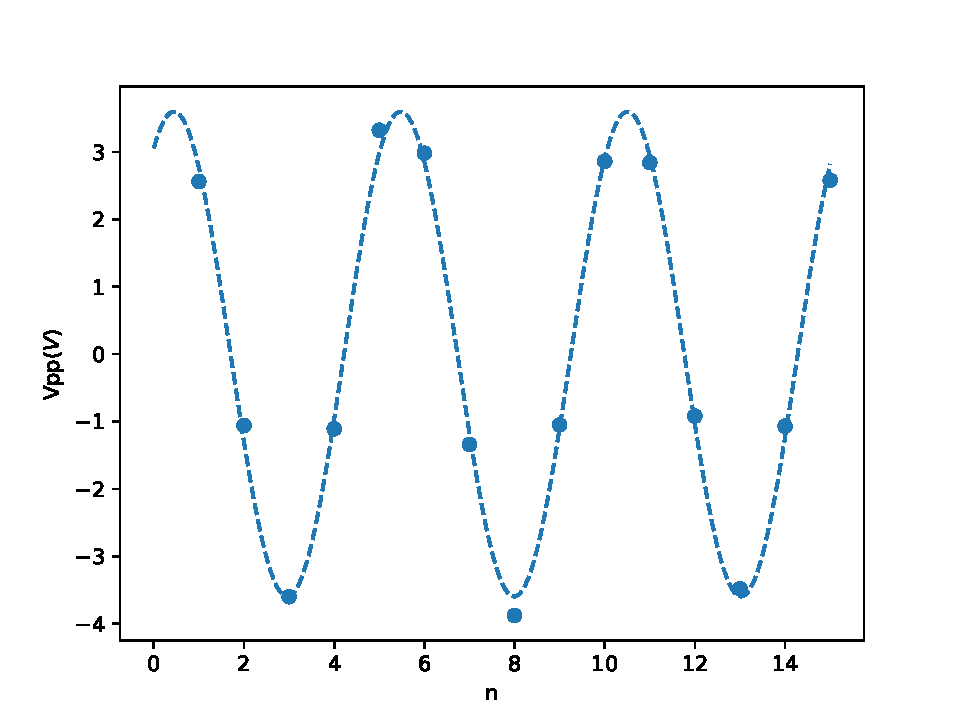
\includegraphics[width=\linewidth]{2144.pdf}
	\caption{$2.144Hz$}
	\label{fig:2144}
\end{figure}

有了这些数据,我们就可以验证色散关系了。根据\ref{eq:1},我们两边平方,选择验证$\omega^2$与$\sin^2(\frac{k}{2})$的线性关系,如图\ref{fig:omegasink}所示。可以看到,我们的数据计算出的$\sin^2(\frac{k}{2})$与$\omega^2$之间有非常良好的线性关系(经计算,$r\geq0.99$),说明符合色散关系。在这里,截距$\omega_p^2=20.7$,斜率$4\omega_s^2=470.1$。故$\omega_p=4.55rad/s$,与理论相差2.71\%,$\omega_s=10.84$,与理论相差4.07\%。可见这一理论具有非常高的准确度,理论和实验符合的很好。

\begin{figure}[htbp]
	\centering
	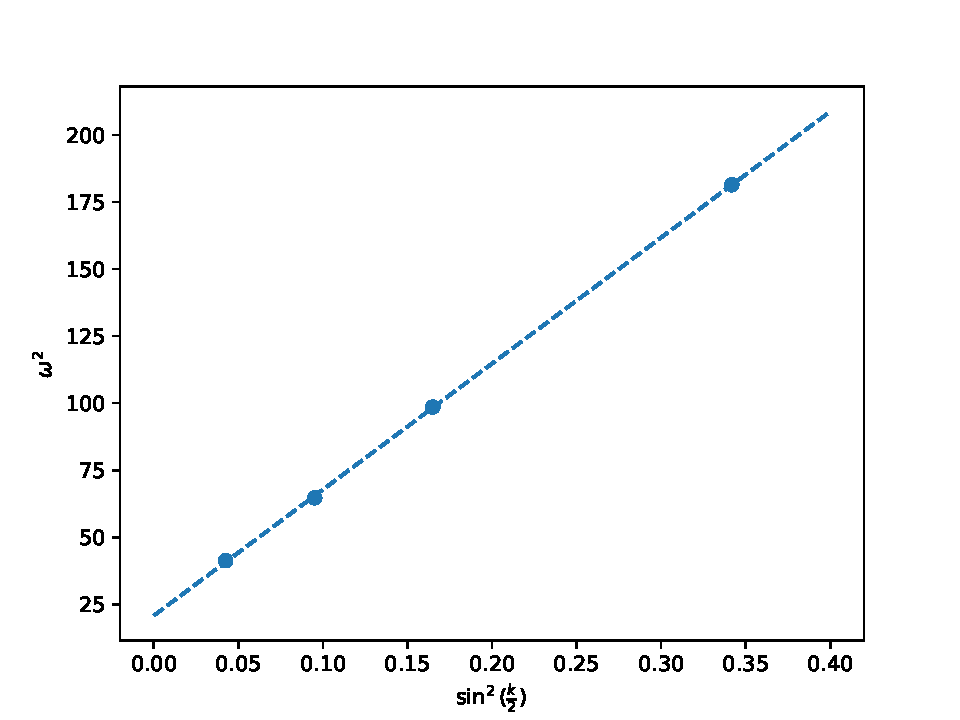
\includegraphics[width=\linewidth]{sin-omega.pdf}
	\caption{色散关系的验证}
	\label{fig:omegasink}
\end{figure}

\subsection{耦合摆通带外的振动特性}

选择低于下限角频率的$0.68Hz$作为驱动频率。低于下限角频率时,可导出振幅呈现$x(n)=Ae^{-cn}$的关系。我们在这样的角频率下用类似于上面的方式测量(此时没有相差,振动方向相同),得到如图\ref{fig:0680}的数据,在这个图中,虚线是用scipy做的指数拟合,拟合得到$A=2.90$,$c=0.126$。

\begin{figure}[htbp]
	\centering
	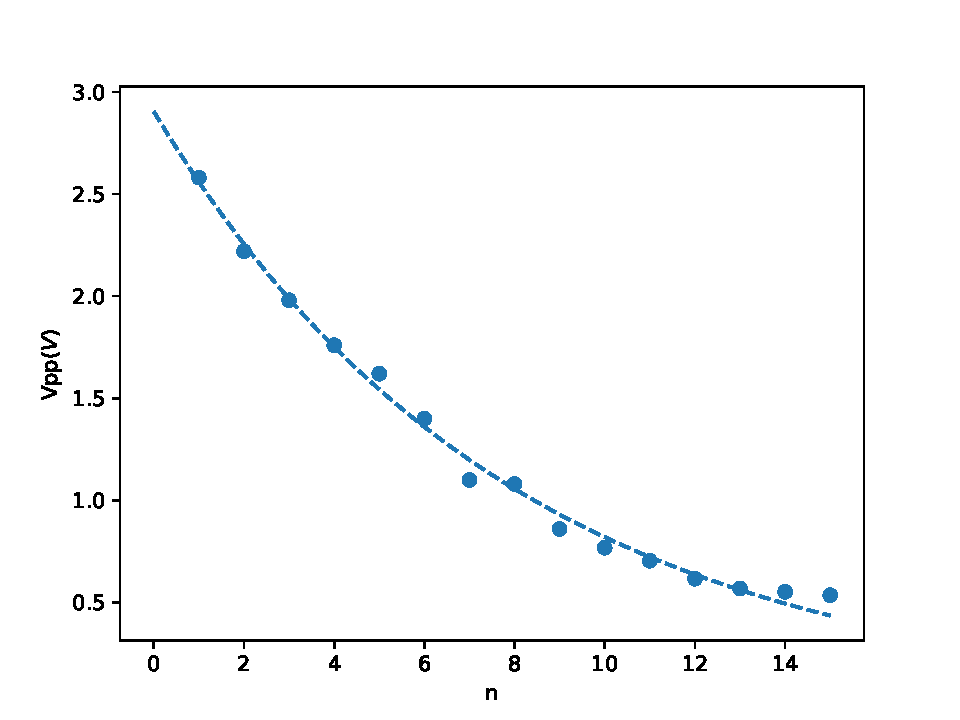
\includegraphics[width=\linewidth]{0680.pdf}
	\caption{通带外的振动}
	\label{fig:0680}
\end{figure}

当然,两边取对数后,上述关系就变成了线性关系,此时做直线拟合($r=-0.991$),结果如图\ref{fig:0680l}。根据拟合出的斜率和截距,求出$A=2.79$,$c=0.121$。可发现跟前面的结果有差距,这是由于优化的函数不同造成的。

\begin{figure}[htbp]
	\centering
	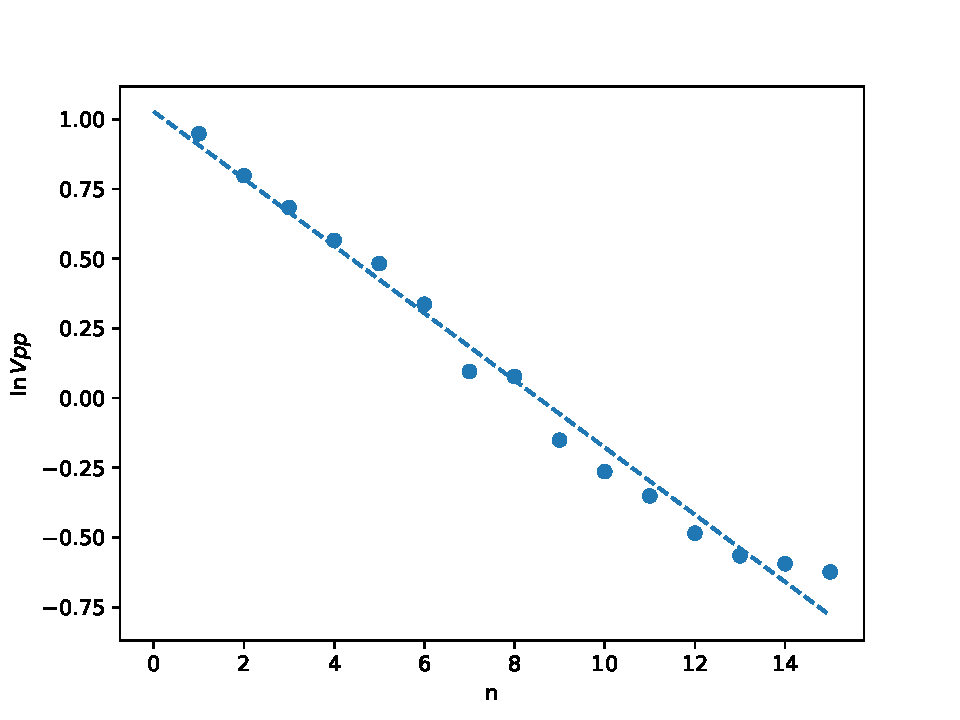
\includegraphics[width=\linewidth]{0680fit.pdf}
	\caption{拟合通带外的振动}
	\label{fig:0680l}
\end{figure}

%------------------------------------------------

\section{讨论}

在前面的实验报告中,我们发现,做数值优化的时候,不同模型,即便同样是最小二乘法,优化出来的结果有差异。实际上是由于数值计算的特点导致的。由于数值计算是离散的逼近,优化算法需要给出特定的初值和优化步数,这样一来,给出的初值和优化步数实际上会导致最终结果的不同。一般情况下,程序有默认的初值和优化步数,不过在某些情况(比如拟合任意函数),自行规定一个区间将会比程序默认得到更好的结果。

%----------------------------------------------------------------------------------------
%	APPENDIX
%----------------------------------------------------------------------------------------

\appendix
\section{附录}
\renewcommand{\thetable}{附表\arabic{table}}
\setcounter{table}{0}

本实验的所有原始数据和代码均上传清华云盘,可点击\href{https://cloud.tsinghua.edu.cn/d/c8e259e22c4d4d68b8cf/}{这个超链接}获得。
%----------------------------------------------------------------------------------------

\end{document}
